\chapter{Conclusiones} 
\label{chapter:conclusiones}

\begin{center}
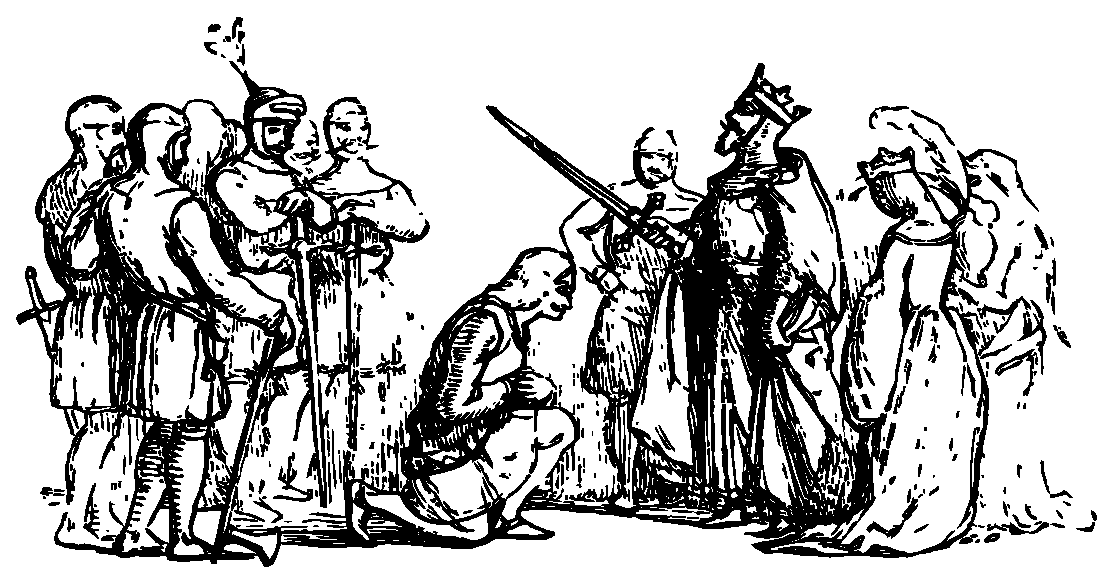
\includegraphics[scale=0.4]{../graphics/johnny_automatic_Jack_and_King_Arthur.eps}
\end{center}

\section{Conclusiones de la implementación}

Implementar las comunidades de práctica con \tiki{} fue una decisión muy importante que tuvimos que sopesar bastante. Sobre todo, cuando estábamos trabajando con un conjunto grande de usuarios y su gestión se tornaba de vital importancia para el éxito del proyecto. Los \profiles{} han resultado ser una herramienta muy útil que ayuda a gestionar la plataforma de una manera bastante cómoda. Entre las alternativas que podemos encontrar en el mercado, no existe un concepto similar y que ofrezca tantas posibilidades como lo hacen éstos en \tiki{}.

Si hay algo que es importante a tener en cuenta es, que las nuevas tecnologías deben ir siempre un paso por delante y tienen que promover, por encima de todas las cosas, la facilidad de uso. Hay muchos colectivos que no están tan implicados, al menos no de una manera tan profunda, con las nuevas tecnologías y son a ellos a los que más hay que tener presente cuando se piensa en crear una nueva interfaz de usuario. Es evidente que \tiki{} tiene que mejorar en múltiples aspectos, sobre todo en la facilidad de uso. También lo tiene que hacer en la propia herramienta de los \profiles{}, puesto que, aún se tiene que aprender a utilizar \yaml{} y eso es algo que no está al alcance de todo el mundo. 

Las conclusiones positivas que se extraen de este trabajo realizado son varias:

\begin{itemize}
\item Se ha conseguido implementar el proyecto \alma{} con bastante éxito y tal cual se pedía en los requisitos. Prueba de ello es que se está utilizando de manera real con un grupo de usuarios considerable en algunas asignaturas impartidas en la \textsc{uah} (en la \figureref{demostracion_alma} se puede ver una captura).
\item Se han mejorado considerablemente las tareas administrativas por parte de un administrador respecto a la que ofrecía originalmente el flujo de trabajo sin \profiles{}. Y esa mejora repercute en una cosa: \textit{productividad}.
\item Estamos contentos de haberlo implementado en \tiki{} (pese a que no es el \textit{software} perfecto, ahora veremos porqué), ya que, esta herramienta, aúna a la vez simplicidad y complejidad. Simplicidad porque es un programa que nada más instalarlo, se puede usar sin mayor complicación. Complejidad porque como hemos visto, se ha comportado de manera excelente a la hora de buscar \q{casos de uso} más complejos.
\end{itemize}

\begin{figure}
\centering
\includegraphics[width=\linewidth]{../graphics/fig_demostracion_alma.png}
\caption{Implementación real de \textsc{alma} con \tiki{}.}\label{fig:demostracion_alma}
\end{figure}

Por contra, en los aspectos negativos nos encontramos que:

\begin{itemize}
\item Uno de los requisitos que pedíamos cuando estábamos buscando un \textit{software} para implementar las comunidades de práctica era: \textit{la instalación y el manejo de la plataforma debe de ser sencillo}. Este hecho, nos limitó un poco el campo de búsqueda de aplicaciones que pudieran crear, hipotéticamente, un gran colectivo de usuarios trabajando con las comunidades de práctica. Todas las aplicaciones que analizamos están basadas en \php{} por ser, precisamente, uno de los lenguajes más fáciles de aprender y de instalar en un servidor. Pero, hay otras plataformas programadas en otros lenguajes de programación como \textsc{java} y que son bastante más potentes que las que hay en \php. Entre muchas propuestas nos encontramos a  \textit{Liferay} \cite{web:liferay} o \textit{Alfresco} \cite{web:alfresco} y que se utilizan, sobre todo, en entornos empresariales. Éstos \cms{} tienen una muy buena implementación del concepto de grupos y recursos y una interfaz de usuario bastante más amigable que la que ofrece \tiki{}. Quizá, implementar las comunidades de práctica en esas plataformas hubiera sido más sencillo que hacerlo en \tiki{} (aún sin contar con los \profiles{}), pero, eso si, aumentando considerablemente la dificultad de modificación del código fuente en dichas aplicaciones (requieren tener un buen conocimiento interno de su estructura, que es infinitamente más compleja que la que utiliza \tiki{}).

\item La herramienta de los \profiles{} aún está en construcción y, debido a esto, las especificaciones de los \textit{Handlers} cambian con bastante frecuencia (aunque cada vez menos). Actualmente se están centrando en mejorar la experiencia de usuario para permitir que cualquier persona pueda usarlos y lo haga sin mucho esfuerzo. Quizá, si hubiéramos esperado más tiempo a la hora de ejecutar este proyecto, es bastante posible que la creación de los \profiles{} se hubiera realizado a \textit{golpe de ratón} en lugar de a \textit{golpe de \yaml{}}.

\end{itemize}

\section{Lecciones aprendidas}

Este \pfc{} ha tenido una duración aproximada de unos dos años (desde que se comenzó a plantear la idea hasta que se ha definió el objetivo concreto), y durante ese tiempo han sucedido múltiples eventos que han servido al autor para aprender en muchos ámbitos. Una de las mayores noticias fue la aceptación por parte de Google para participar en su programa \textit{Summer of Code} de 2009 en la mejora de los \textit{Workspaces} (que no es un concepto bastante parecido al de las comunidades de práctica) de \tiki{}. Entre otras cosas se aprendió:

\begin{itemize}

\item Como se organiza una plataforma de código abierto (su arquitectura interna) y como los recursos humanos son coordinados para la consecución de un objetivo común.

\item A mejorar las habilidades codificando con \php{}. Al comenzar el proyecto desconocía cómo se programaba en este lenguaje y, al acabarlo, puedo decir orgulloso que es uno de los que más conozco.

\item A mejorar mi nivel de inglés. Estar en un ambiente de índole internacional me permitió conocer nueva gente y a expresar mis ideas dando charlas en público.

\item A aprender el maravilloso mundo de la tipografía y la maquetación. Maquetar un libro es una tarea que no es trivial y que requiere un esfuerzo y unas ganas por aprender bastante importantes. El resultado que has podido ver (y leer), es fruto de todo este esfuerzo.

\end{itemize}

\section{Futuras lineas de trabajo}

Hay que reconocer que, aunque durante todo este \pfc{} se han estado ensalzando las virtudes de \tiki{}, éste posee unas serie de desventajas considerables en cuanto a varios aspectos de la plataforma. La verdad sea dicha, hay bastantes cosas que se pueden enriquecer aún más y que son susceptibles de que alguien coja el testigo y las convierta en realidad, entre ellas destacamos (sin ningún orden concreto de prioridad):

\begin{enumerate}

\item Mejorar las interfaces gráficas de administración de \profiles{} de \tiki{}. Actualmente los \profiles{} requieren que una persona tenga ciertos conocimientos técnicos a la hora de poder implementarlos. Eso en un entorno docente puede ser que no sea factible, quizá un profesor está al cargo de alguna asignatura y por el mero hecho de que ni si quiera sabe qué es \yaml{} no debería ser discriminado. ¿De qué manera podríamos solucionar este problema? Actualmente Apple \cite{web:apple} en su sistema operativo \textsc{os x} \cite{web:apple-os-x} tiene una herramienta llamada \textit{Automator} \cite{web:apple-automator} que enmascara a un usuario que no sabe de programación la tarea de crear pequeños programas que hagan ciertas tareas (conocidos como \textit{flujos de trabajo}). Para crear un nuevo programa el usuario simplemente tiene que ir arrastrando pequeños componentes que realizan una acción concreta (por ejemplo, \q{listar todos los documentos en un directorio}) e ir uniendo más componentes al flujo (podría añadir: \q{seleccionar aquellos ficheros que tengan formato \textsc{pdf}}) hasta que obtiene un programa que realiza una tarea concreta (podría finalizar el flujo añadiendo: \q{y mover dichos archivos a la carpeta de mis documentos}). En la \figureref{flujo_trabajo_automator} podemos ver el flujo real que se ha comentado antes. En \tiki{} se podría realizar algo similar con los \profiles{} y eso es algo que una persona que no tiene muchos conocimientos técnicos, puede asumirlo y aprender a usarlo.

\item Los \profiles{} que se han creado son muy \q{rígidos}, y asumen muchas cosas por defecto (por ejemplo sólo crea una \textit{wiki}, pero no crea un foro). Se podrían crear más \profiles{} que abarquen más casos de uso.

\item El sistema de los \textit{Data Channels} no tiene una implementación muy clara. Sería útil crear un apartado en \tiki{} donde se pudieran guardar los \textit{Data Channels} creados al igual como se listan los recursos en las categorías. Esto permitiría mejorar la facilidad de uso de la plataforma.

\item Enriquecer y adaptar la documentación que se encuentra en: \url{http://doc.tiki.org}. Muchas veces cuando un usuario necesita saber cosas concretas de la plataforma tiene que acudir a la documentación oficial para aclarar sus dudas. El problema es que en muchas áreas ésta no está de forma clara o incluso contiene información anticuada de anteriores versiones que ya no es vigente y que no sirve. Mejorar la documentación ayudaría a que los usuarios tuviesen un mejor conocimiento de la plataforma.

\item La traducción al castellano del propio \tiki{} es irregular y, en ocasiones, de mala calidad: se entremezclan oraciones en inglés con algunas en castellano. De cara a mostrar una buena imagen, se debería traducir de forma correcta.
\end{enumerate}

\begin{figure}
\centering
\includegraphics[width=\linewidth]{../graphics/fig_flujo_trabajo_automator.png}
\caption{Ejemplo del programa Automator.}\label{fig:flujo_trabajo_automator}
\end{figure}